\documentclass[a4paper, 11pt]{thesis}

/stock/16_git_repo/library/library.tex

\newcommand{\openord}[1]{\begin{center}\begin{ganttchart}[hgrid=true,vgrid={{dotted}},inline]{#1}
    \gantttitlelist{1,...,#1}{1}\\}
\newcommand{\closeord}{\end{ganttchart}\end{center}}

% marin.bougeret@lirmm.fr
% Possibilités de thèse à Grenoble pour de l'ordonnacement

\begin{document}

\chapter{R\'{e}sultats positifs (FPTAS)}

\section{Préliminaires}

\subsection{Notations}

\subsubsection{Notation à trois champs}

La notation à trois champs est une notation de la forme :
\begin{displaymath}
    \begin{array}{c|c|c}
        P & & \\
        Q & & c_{max} = \sum c_i \\
        R & & \\
          & & \\
        \mbox{Machines} & \mbox{Contraintes} & \mbox{Fonction objectif} \\
    \end{array}
\end{displaymath}

\begin{rmq}
    ~\\Dans cette notation, le premier champs peut prendre trois valeurs :
\begin{itemize}
    \item $Q$ chaque machine $i$ a une vitesse $s_i$. Ordonnancer la tâche $j$ sur $i$ nécessite
        $\frac{p_j}{s_i}$ unités de temps.
    \item $R$ plus général, le temps est donné par $x_{ij}$
    \item $P$ toutes les machines sont identiques\\
\end{itemize}
\end{rmq}

\begin{ex}[$P | C | C_{MAX}$]

~\\Étant donné, $m$ machines identiques, $n$ tâches indépendantes\footnote{Pas de règles de
priorités ou d'exécutions pré-requises.} avec $p_j$ la durée de la tâche $j$.
On cherche à ordonnancer les $n$ tâches sur les $m$ machines (sans préemptions) pour minimiser
$\max_{1 \leq j \leq n} C_j$ où $c_j$ est le "completion time" de la tâche $j$ \footnote{makespan,
noté $C_{max}$}.\\
\end{ex}

\subsection{Définitions}

\subsubsection{NP-hard sens fort, sens faible}

On considère $\Pi_{dec}$ :

\textbf{Entrée :} $x_i, 1 \leq i \leq n$ avec $\forall i, 0 \leq x_i \leq C$

\textbf{Question :}

% figure 10

\subsection{Différents problèmes}

\section{Analyse classiques de gloutons}

\subsection{Technique de SWAP et de restructuration d'un optimal}

Exemple sur $1 | | \sum\omega_jc_j$. On a une machine, chaque tâche a : \begin{displaymath}
\left \lbrace \begin{array}{rcl}
    p_j & : & \mbox{processing time} \\
    \omega_j & : & \mbox{poids} > 0 \\
\end{array} \right .\end{displaymath}

On cherche à minimiser $\sum_{j =1}^n \omega_j c_j$.\\

\begin{ex}
    ~\\ On définit deux taches comme suit : 
    \begin{displaymath}
        \begin{array}{|c|c|c|}\hline
            c_1 & p_1 = 4 & \omega_1 = 2 \\ \hline
            c_2 & p_2 = 2 & \omega_2 = 2 \\ \hline
        \end{array}
    \end{displaymath}

    Considérons l'ordonnancement suivant : 

    \openord{7}
        \ganttbar{$c_2$}{1}{2}
        \ganttbar{$c_1$}{3}{6}
    \closeord
\end{ex}

En exécutant $c_2$ en premier, le coût est donné par : \begin{displaymath}
\begin{array}{rcl}
    \mbox{coût} & = & 2 \times 2  + 2 \times 6\\
                & = &  16\\
\end{array} \end{displaymath}

Le coefficient $6$ est la date de fin de $c_1$.

\subsubsection*{Intuition}
Si tous les $\omega_j = 1$ :
\begin{displaymath}\begin{array}{rcl}
    \mbox{coût} & = & c_1 + c_2 + c_3 \\
                & = & p_1 + (p_1 + p_2) + (p_1 + p_2 + p_3) \\
                & = & 3p_1 + 2p_2 + p_3 \\
\end{array} \end{displaymath}

Quand $\omega_j = 1$, on s'aperçoit qu'il faut ordonner par $p_j$ croissant\footnote{SPT : Shortest
processing time (first)}

Si $\forall j=1, \dots n,\quad p_j = 1$ 
Le coût est alors donné par $\mbox{coût} = \omega_1 + 2\omega_2 + 3\omega_3$, on cherchera donc à
ordonnancer par $\omega_j$ décroissant.

Il existe un algorithme polynomial pour $1 | | \sum\omega_jc_j$, il s'agit de "SMITH RULE" :\\
Ordonnancer par $\frac{p_j}{\omega_j}$ croissant.

\subsubsection*{Preuve : SMITH RULE est optimale}

\begin{lemma}
    Soit $S$ une solution de la forme :

    \openord{20}
        \ganttbar[bar/.style={fill=black}]{}{1}{8}
        \ganttbar{$c_1$}{9}{10}
        \ganttbar{$c_2$}{11}{12}
        \ganttbar[bar/.style={fill=black}]{}{13}{20}
    \closeord

    Si : \begin{displaymath}
    \frac{p_2}{\omega_2} \leq \frac{p_1}{\omega_1} \end{displaymath}
    Alors il existe $S'$ de la forme : 

    \openord{20}
        \ganttbar[bar/.style={fill=black}]{}{1}{8}
        \ganttbar{$c_2$}{9}{10}
        \ganttbar{$c_1$}{11}{12}
        \ganttbar[bar/.style={fill=black}]{}{13}{20}
    \closeord 

    telle que $\mbox{coût}(S') \leq \mbox{coût}(S)$
\end{lemma}

\begin{proof}
    \begin{displaymath} \begin{array}{rrcl}
        & \mbox{coût}(S) & = &  X + \omega_1(t + p_1) + \omega_2(t + p_1 + p_2) + Y \\
        & \mbox{coût}(S') & = & X + \omega_2(t + p_2) + \omega_1(t + p_2 + p_1) + Y \\
        \Rightarrow & \Delta & = & \mbox{coût}(S) - \mbox{coût}(S') \\
                    & & = & \omega_2 p_1 - \omega_1 p_2 \geq 0 \\
    \end{array} \end{displaymath}

    Car $\omega_2 p_1 \geq \omega_1 p_2$
\end{proof}

\begin{lemma}[Restructuration optimale]
    Soit OPT, $\exists S_1, S_2, \dots, S_r$ : \begin{displaymath}
    \begin{array}{rcl}
        \mbox{coût}(OPT) & \geq & \mbox{coût}(S_1) \\
                         & \geq & \mbox{coût}(S_r) \\
    \end{array} \end{displaymath}
\end{lemma}

% fig 8
% Rattraper la figure 8 (il manque un morceau de preuve)

\subsubsection*{Exemple : $P2 | | C_{max}$}

\begin{center}
\begin{ganttchart}[hgrid=true,vgrid={{dotted}},inline,today=5,today label=$C_{max}$]{6}
    \gantttitlelist{1,...,6}{1}\\
    \ganttbar{$c_2$}{1}{2}
    \ganttbar{$c_3$}{3}{4} \\
    \ganttbar{$c_2$}{1}{1}
    \ganttbar{$c_4$}{2}{5} 
\end{ganttchart}
\end{center}

\begin{thrm}
    $P2 | | C_{max}$ est NP-hard
\end{thrm}

\begin{proof}
On fait une réduction à partir de $2-$partition :

\textbf{Données :} Un ensemble d'éléments $S = \{x_i,~ 1 \leq i \leq n\}$, une fonction $\omega$ à
valeurs dans $\mathbb{N}$ affectant un poids à chacun des éléments de $S$ :
\begin{displaymath}
    \omega \left \lbrace \begin{array}{rcl}
        S & \longrightarrow & \mathbb{N}\\
        x_i & \longmapsto & \omega(x_i)
    \end{array} \right .
\end{displaymath}
On pose, sans perte de généralité : $\sum_S x_i = 2a$

\textbf{Question :} Est il possible de partitonner $S$ en deux sous ensembles $S_1$ et $S_2$ tels
que : \begin{itemize}
    \item $S_1 \cap S_2 = \emptyset$ 
    \item $S_1 \cup S_2 = S$
    \item $\sum_{S_1} = \sum_{S_2} = a$\\
\end{itemize}

Il est possible à partir d'une instance quelconque de $2-$partition de construire une instance de
$P_2| | C_{max}$ de la manière suivante : \begin{itemize}
    \item $n$ tâches
    \item chaque tâche $j$ est telle que $p_j = x_j$\\
\end{itemize}
S'il existait un algorithme polynomial permettant de résoudre $P_2| | C_{max}$, on pourrait alors
résoudre $2-$partition en temps polynomial en répondant OUI s'il existe un ordonnancement tel que
$C_{max} \leq a$ et non sinon.
\end{proof}

\begin{rmq}
    $P2 || C_{max}$ est NP-hard sens faible
\end{rmq}

On va résoudre $\overline{P_2 | | C_{max}}$ en temps $\poly(n)$ en utilisant la programmation dynamique.

$PD(j, l_1, l_2) =$ étant donné que la machine $i$ est chargée de $0$ à $l_i$, $PD(j, l_1, l_2)$
ordonnance les tâches $j, \dots, n$ de façon optimale.

\begin{algorithm}[h!]
    \caption{Programmation dynamique}
    \label{pd_p2cmax}
    \begin{algorithmic}[1]
        \Function{PD}{$j, l_1, l_2$}
            \If{$j = n + 1$}
                \State \Return $\max(l_1, l_2)$;
            \Else
                \State \Return $\min(PD(j+1, l_1 + p_j, l_2), PD(j+1, l_1, l_2 + p_j))$;
            \EndIf
        \EndFunction
    \end{algorithmic}
\end{algorithm}

$PD(1, 0, 0)$ donne une solution optimale en temps $O(n^3c^2)$.
Pour la programmation dynamique, la complexité est donnée par le nombre de valeurs possibles des
paramètres multiplié par le temps d'exécution d'un traitement. Le nombre de valeurs possibles est
donné par : \begin{displaymath}
\begin{array}{rrcl}
    1 \leq j \leq n \ & 0 & \leq l_1 \leq & n \times \max(p_j) = nc \\
    nx \ & (nc)^2 \\
\end{array}\end{displaymath}

Dans le cas général (pour $P2 || C_{max}$), cet algorithme est pseudo polynomial, c'est à dire 
$\poly(n, C)$. Et donc, si on se restreint à $\overline{P2 || C_{max}}$, $C = \poly(n)$ et l'algorithme devient
polynomial.

\begin{rmq}
    Un problème NP-hard sens fort ne peut pas avoir d'algorithme pseudo polynomial\footnote{Sauf si $P =
    NP$}
\end{rmq}

\begin{rmq}
    $\forall 0 \leq x \leq nC$, on lance $S_1 = KP(\mbox{taches}, x)$\footnote{KP = Knapsac Problem,
    sac à dos} et $S_2 = \{1, \dots, n\} \backslash S_1$ on obtient une solution $\sigma_x$.
    On retourne alors la meilleure solution de $\sigma_x$ pour $1 \leq x \leq nC$
\end{rmq}

\begin{thrm}
    $P || C_{max}$ est NP-hard (sens fort)
\end{thrm}


\begin{proof}
    On fait une réduction depuis $3-$partition :

    \textbf{Données :} Un ensemble d'éléments $S = \{x_i, 1 \leq i \leq n\}$, une fonction $\omega$
    à valeurs dans $\mathbb{N}$ affectant un poids à chacun des éléments de $S$ :
    \begin{displaymath}
        \omega \left \lbrace \begin{array}{rcl}
            S & \longrightarrow & \mathbb{N} \\
            x_i & \longmapsto & \omega(x_i) \\
        \end{array} \right .
    \end{displaymath}

    \textbf{Question :} Étant donné $x_j, 1 \leq j \leq n$, peut on partitionner les $x_j$ en $\frac{n}{3}$ triplets $x_1^l,
    x_2^l, x_3^l, 1 \leq l \leq \frac{n}{3}$. 
    
    On a $\sum_{j = 1}^n x_j = \frac{na}{3}$, donc $\sum_{t=1}^3 x_t^l = a$, on pose alors $m =
    \frac{n}{3}$ machines, $n$ tâches $p_j = x_j$, si $3-$partition retourne oui, alors
    $OPT_{P||C_{max}} \leq a$

    % figure 13
    \begin{center}
    \begin{tikzpicture}
        \draw (0,5) rectangle (3, 4.5);
        \draw (3,5) rectangle (4, 4.5);
        \draw (4,5) rectangle (7, 4.5);
        \draw (0,4) rectangle (4, 3.5);
        \draw (4,4) rectangle (5.5, 3.5);
        \draw (5.5, 4) rectangle (7, 3.5);
        \filldraw [black]   (3.5, 2) circle (1pt)
                            (3.5, 2.5) circle (1pt)
                            (3.5, 3) circle (1pt)
                            (3.5, 1.5) circle (1pt);
        \draw (0,1) rectangle  (2, 0.5);
        \draw (2, 1) rectangle (6, 0.5);
        \draw (6, 1) rectangle (7, 0.5);
        \draw (7, 5.5) -- (7, 0);
        \draw (7, 6) node {$a$};
        \draw[<->] (0, 5.6) to (3.5, 5.6) node[anchor=south] {$a$} to (7, 5.6);
    \end{tikzpicture}
    \end{center}

    S'il retourne non, alors $OPT_{P||C_{max}} \geq a + 1$
\end{proof}

\subsection{$2-\frac{1}{m}$ approximation pour $P||C_{max}$}

On va définir l'algorithme "List Scheduling" (LS) :
\begin{algorithm}[h!]
    \caption{List Scheduling}
    \label{alg_ls}
    \begin{algorithmic}[1]
        \Function{LS}{$t_1, \dots, t_n$}
            \State Ordonner les tâches selon un critère de son choix;
            \For{$1 \leq i \leq n$}
                \State ordonnancer la tâche $i$ pour qu'elle termine le plus tôt possible;
            \EndFor
        \EndFunction
    \end{algorithmic}
\end{algorithm}

\begin{ex}
    Le nombre de machines $m$ est fixé à $3$. La liste des tâches triées par ordre dichotomique est
    la suivante :

\begin{center}
    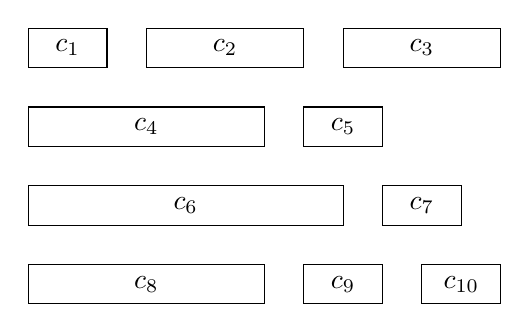
\begin{tikzpicture}[scale=0.5]
        \draw (0, 9) rectangle (2, 8);
        \draw (3, 9) rectangle (7, 8);
        \draw (8, 9) rectangle (12, 8);

        \draw (0, 7) rectangle (6, 6);
        \draw (7, 7) rectangle (9, 6);

        \draw (0, 5) rectangle (8, 4);
        \draw (9, 5) rectangle (11, 4);

        \draw (0, 3) rectangle (6, 2);
        \draw (7, 3) rectangle (9, 2);
        \draw (10, 3) rectangle (12, 2);

        \draw (1, 8.5) node {$c_1$};
        \draw (5, 8.5) node {$c_2$};
        \draw (10, 8.5) node {$c_3$};

        \draw (3, 6.5) node {$c_4$};
        \draw (8, 6.5) node {$c_5$};

        \draw (4, 4.5) node {$c_6$};
        \draw (10, 4.5) node {$c_7$};

        \draw (3, 2.5) node {$c_8$};
        \draw (8, 2.5) node {$c_9$};
        \draw (11, 2.5) node {$c_{10}$};
    \end{tikzpicture}
\end{center}

L'ordonnacement correspondant :
\openord{8}
    \ganttbar{$c_1$}{1}{1}
    \ganttbar{$c_4$}{2}{4}
    \ganttbar{$c_8$}{5}{7} \\
    \ganttbar{$c_2$}{1}{2} 
    \ganttbar{$c_5$}{3}{3}
    \ganttbar{$c_7$}{4}{4}
    \ganttbar{$c_9$}{5}{5}
    \ganttbar{$c_{10}$}{6}{6} \\
    \ganttbar{$c_3$}{1}{2}
    \ganttbar{$c_6$}{3}{6}
\closeord
\end{ex}

\begin{prop}
    List Scheduling est une $2 - \frac{1}{m}$ approximation pour $P||C_{max}$.
\end{prop}

\begin{proof}
    Soit $x$ une tâche qui atteint le makespan, soit $s_x$ la date de début de $x$,
    on a donc $ LS = s_x + p_x $. Par définition de $LS$, $\forall t \in [0, s_x]$, toutes les machines
    travaillent.

    Soit :
    \begin{displaymath}
        W = \sum_{j=1}^n p_j$, $W \geq m s_x + P_x \Rightarrow s_x \leq \frac{W - p_x}{m}
    \end{displaymath}
    donc : \begin{displaymath}
    \begin{array}{rcl}
        LS & \leq & \displaystyle \frac{W - p_x}{m} + p_x \\
           & = & \displaystyle \frac{W}{m} + p_x \left ( 1 - \frac{1}{m} \right )
    \end{array}
    \end{displaymath}
\end{proof}

\begin{lemma}[Bornes inférieures classiques]
    Voici quelques bornes classiques :
    \begin{itemize}
        \item $\frac{W}{m} \leq OPT$
        \item $p_x \leq OPT$
    \end{itemize}
\end{lemma}

On a donc : \begin{displaymath}
LS \leq OPT \left ( 2 - \frac{1}{m} \right ) \end{displaymath}

\begin{thrm}
    La borne est tight (= atteinte)
\end{thrm} 

\begin{proof}
\textbf{Intuition :} Le tri peut être mauvais et une tâche très grande peut être mise tout à la fin
de l'ordonnacement. On se retrouverait alors dans un cas de figure de ce genre :

\openord{10}
    \ganttbar[bar/.style={fill=black}]{}{1}{4} 
    \ganttbar{$c_k$}{5}{9} \\
    \ganttbar[bar/.style={fill=black}]{}{1}{4} \\
    \ganttbar[bar/.style={fill=black}]{}{1}{4} \\
    \ganttbar[bar/.style={fill=black}]{}{1}{4} \\
    \ganttbar[bar/.style={fill=black}]{}{1}{4} 
\closeord

On prend une tâche de taille $m$ et $m(m - 1)$ tâches de taille $1$. Si LS trie par $p_j$ croissant,

% figure 16
\begin{center}
    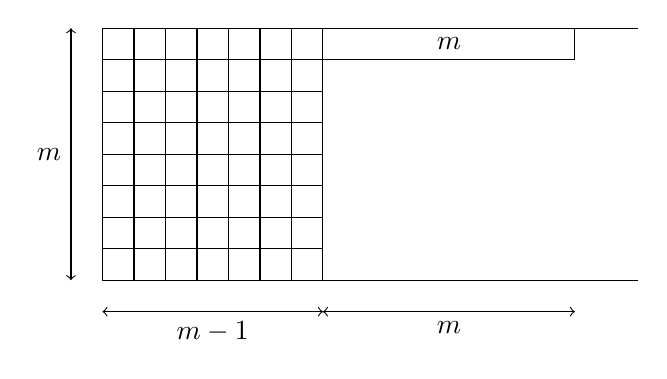
\begin{tikzpicture}[scale=0.4]
        \foreach \x in {0,1,...,7}
            \draw (\x, 8) -- (\x, 0);
        \foreach \y in {0,1,...,8}
            \draw (0, \y) -- (7, \y);
        \draw (0, 8) -- (17, 8);
        \draw (0, 0) -- (17, 0);
        \draw (7, 8) rectangle (15, 7);
        \draw (11, 7.5) node {$m$};
        \draw[<->] (0, -1) -- (3.5, -1) node[anchor=north]{$m-1$} -- (7, -1);
        \draw[<->] (7, -1) -- (11, -1) node[anchor=north]{$m$} -- (15, -1);
        \draw[<->] (-1, 8) -- (-1, 4) node[anchor=east]{$m$} -- (-1, 0);

    \end{tikzpicture}
\end{center}

$OPT = m,\quad LS = 2 m - 1 \Rightarrow \rho = \frac{2m -1}{m} = 2 - \frac{1}{m}$
\end{proof}

\begin{thrm}
    Soit LPT\footnote{Longest Processing Time (first)} = LS où l'on trie par $p_j$ décroissant.
    LPT est une $\left (\frac{4}{3} - \frac{1}{3m})\right )$ approximation.
\end{thrm}

\textbf{Intuition :} "Taquiner la formule"

\begin{displaymath}\begin{array}{rcl}
LS & \leq & \displaystyle \frac{W}{m} + p_x \\
   & \leq & OPT \\
\end{array}
\end{displaymath}

Le résultat est trivial si $\displaystyle p_x \leq \frac{OPT}{3}$.


\begin{proof}
    Soit $x$ la tâche qui atteint le makespan de LPT.
    $W \leq ms_x + p_x \quad \mbox{avec} \quad s_x \leq \frac{W - p_x}{m}$ \\

    \begin{displaymath} \begin{array}{rcl}
        LPT & \leq & s_x + p_x \\
            & \leq & \displaystyle \frac{W}{m} + p_x \left (1 - \frac{1}{m} \right )\\
    \end{array} \end{displaymath}
\end{proof}

% figure 17
\begin{center}
    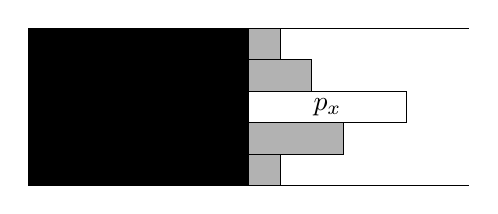
\begin{tikzpicture}[scale=0.4]
        \filldraw (0, 5) rectangle (7, 0);
        \draw[fill=black!30] (7, 5) rectangle (8, 4);
        \draw[fill=black!30] (7, 4) rectangle (9, 3);
        \draw[fill=black!30] (7, 2) rectangle (10, 1);
        \draw[fill=black!30] (7, 1) rectangle (8, 0);
        \draw (7, 3) rectangle (12, 2);
        \draw (9.5, 2.5) node {$p_x$};
        \draw (0, 5) -- (14, 5);
        \draw (0, 0) -- (14, 0);
    \end{tikzpicture}
\end{center}

\begin{itemize}
    \item Cas 1 : si $p_x \leq \frac{OPT}{3}$\\
        \begin{displaymath} \begin{array}{rcl}
            LPT & \leq & OPT + \frac{OPT}{3} \left ( 1 - \frac{1}{m} \right ) \\
                & \leq & OPT \left( \frac{4}{3} - \frac{1}{3m} \right ) \\
        \end{array} \end{displaymath}
    \item Cas 2 : si $p_x > \frac{OPT}{3}$\\
        Soit $I' = \{j / s_j \leq s_x \}$, on a $LPT(I') = LPT(I)$\footnote{On supprime toutes les
        tâches positionnées après $p_x$, qui n'influent pas sur le temps d'exécution optimal.}
        On va montrer que : \begin{displaymath}
        LPT(I) = LPT(I') = OPT(I') \leq OPT(I) \end{displaymath}

        \textbf{Intuition} : Toutes les tâches $j$ avant $x$ vérifient $p_j \geq p_x$ et donc
        $p_j > \frac{OPT}{3} \quad \forall j = 1, \dots, x-1$. Ceci d'écrit : \begin{displaymath}
        \forall j \in I', \quad p_j > \frac{OPT(I')}{3} > \frac{OPT(I)}{3} \end{displaymath}
        On a alors $|I'| \leq 2m $.

        On va prouver que $LPT(I') = OPT(I')$, pour ce faire, quelle est la structure de $OPT(I')$

        %figure 18
\end{itemize}

\section*{Analyse de List Scheduling sur le problème $P | Prec | C_{max}$}

\textbf{Input :} $n$ tâches $p_j$, $m$ machines identiques, Prec est le graphe de
        précédence\footnote{Il s'agit d'un DAG (=Directed Acyclic Graph), s'il existe une arête
        $j_1j_2$ dans l'arbre, alors la tache $j_1$ doit être terminée pour que $j_2$ commence.}
\begin{center}
    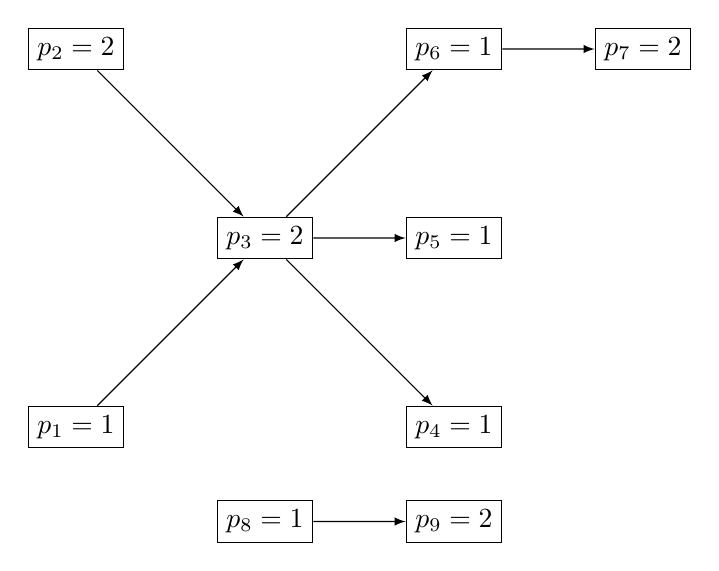
\begin{tikzpicture}[scale=0.6, prec/.style={<-, >=latex}]
        \tikzset{tache/.style={rectangle, minimum height=0.5cm, minimum width=1cm, draw=black}};
        \node[tache] (1) at (0, 0) {$p_1 = 1$};
        \node[tache] (2) at (0, 8) {$p_2 = 2$};
        \node[tache] (3) at (4, 4) {$p_3 = 2$}
            edge[prec] (1)
            edge[prec] (2);
        \node[tache] (6) at (8, 8) {$p_6 = 1$}
            edge[prec] (3);
        \node[tache] (5) at (8, 4) {$p_5 = 1$}
            edge[prec] (3);
        \node[tache] (4) at (8, 0) {$p_4 = 1$}
            edge[prec] (3);
        \node[tache] (7) at (12, 8) {$p_7 = 2$}
            edge[prec] (6);

        \node[tache] (8) at (4, -2) {$p_8 = 1$};
        \node[tache] (9) at (8, -2) {$p_9 = 2$}
            edge[prec] (8);
    \end{tikzpicture}
\end{center}

\textbf{Output :} Un ordonnancement des tâches minimisant le temps total d'exécution.

\openord{9}
    \ganttbar{$8$}{1}{1}
    \ganttbar{$9$}{2}{3}
    \ganttbar{$5$}{6}{6}\\
    \ganttbar{$1$}{1}{1}
    \ganttbar{$2$}{2}{3}
    \ganttbar{$3$}{4}{5}
    \ganttbar{$4$}{6}{6}
    \ganttbar{$6$}{7}{7}
    \ganttbar{$7$}{8}{8}
\closeord

On définit le \emph{List Scheduling} pour un graphe :

\begin{algorithm}[h!]
    \caption{List Scheduling sur Graphe}
    \label{alg_ls_g}
    \begin{algorithmic}[1]
        \While{Pas Fini}
            \State Prendre une tâche prête;
            \State L'ordonnancer au plus tôt;
        \EndWhile
    \end{algorithmic}
\end{algorithm}

\begin{thrm}
    LS est une $2 - \frac{1}{m}$ approximation pour $P|Prec|C_{max}$
\end{thrm}

Considérons l'ordonnancement réalisé par LS :

\begin{center}
    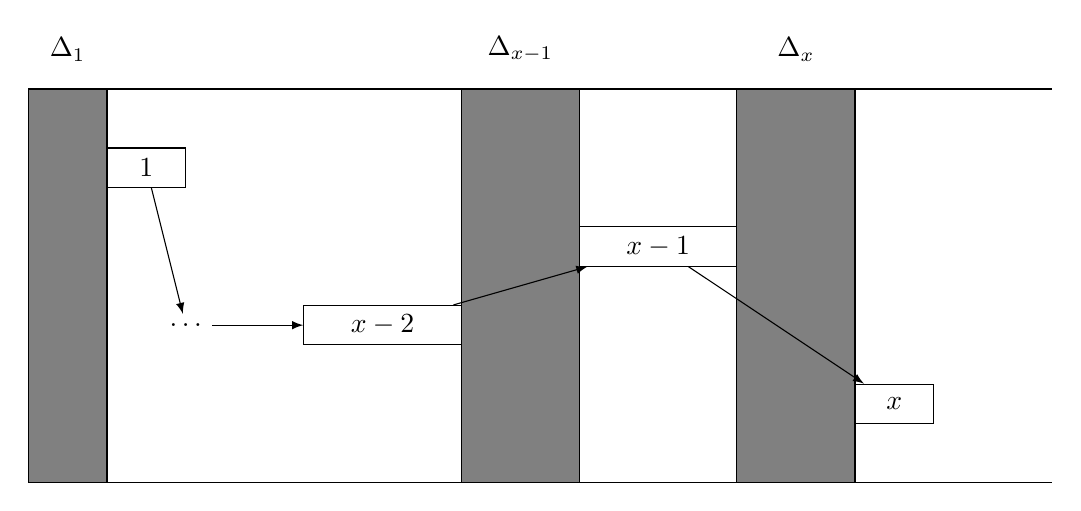
\begin{tikzpicture}[prec/.style={<-, >=latex}]
        \tikzset{tache/.style={rectangle, minimum height=0.5cm, minimum width=1cm, draw=black}};
        \draw (0, 0) -- (13, 0);
        \draw (0, 5) -- (13, 5);

        \draw[fill=black!50] (0, 5) rectangle (1, 0);
        \draw[fill=black!50] (5.5, 5) rectangle (7, 0);
        \draw[fill=black!50] (9, 5) rectangle (10.5, 0);

        \node[tache] (t1) at (1.5, 4) {$1$};
        \node (p) at (2, 2) {$\dots$}
            edge[prec] (t1);
        \node[tache, minimum width=2cm] (t2) at (4.5, 2) {$x-2$}
            edge[prec] (p);
        \node[tache, minimum width=2cm] (t3) at (8, 3) {$x-1$}
            edge[prec] (t2);
        \node[tache] (t4) at (11, 1) {$x$}
            edge[prec] (t3);
        
        \node at (0.5,  5.5) {$\Delta_1$};
        \node at (6.25, 5.5) {$\Delta_{x-1}$};
        \node at (9.75, 5.5) {$\Delta_x$};
    \end{tikzpicture}
\end{center}

Soit $x$ une tâche qui atteint le makespan, soit $x - 1$ le dernier prédécesseur de $x$. On sait que
pendant le temps $\Delta_x$, toutes les machines sont occupées\footnote{Sinon on aurait pu lancer
$x$ plus tôt.}. Soit $x-2$ le dernier prédécesseur de $x-1$, de la même manière, pendant
$\Delta_{x-1}$, toutes les machines travaillent. On procède ainsi jusqu'à la tâche $1$.

La valeur de LS est donnée par : \begin{displaymath}
    LS = \sum_{i=1}^x \Delta_i + \sum_{i=1}^x p_i
\end{displaymath}

On pose $\sum_{i=1}^x p_i = C$ que l'on définit comme la taille de la chaîne définie par récursion.
Intéressons nous aux bornes, on voit que $C \leq OPT$ car ($OPT \geq$ chemin critique $+$ longueur de
la chaîne), de plus, on peut écrire : \begin{displaymath}
    W \geq m \sum_{i=1}^x \Delta_i + C
\end{displaymath}

On en déduit : \begin{displaymath}
    \sum_{i=1}^x \Delta_i \leq \frac{W - C}{m}
\end{displaymath}

Donc dans LS, on obtient : \begin{displaymath}
    \begin{array}{rcl}
        LS & \leq & \displaystyle \frac{W - C}{m} + C \\
           & \leq & \displaystyle \frac{W}{m} + C(1 - \frac{1}{m}) \\
           & \leq & \displaystyle \frac{m OPT}{m} + OPT(1 - \frac{1}{m}) \\
           & \leq & \displaystyle OPT(2 - \frac{1}{m})
    \end{array}
\end{displaymath}
La borne est atteinte par le même exemple que précédemment.

\begin{rmq}
    LS sur $Q| | C_{max}$\footnote{Chaque machine a une vitesse différente.}
    On réalise la même analyse et on arrive à : \begin{displaymath}
        LS \leq \frac{W}{\sum_{i=1}^m s_i} + \frac{p_x}{s_{i_0}} \leq \frac{W}{}
        % fig 21
    \end{displaymath}
\end{rmq}

\section{Dual approx}

\begin{df}
    Une $\rho$\footnote{$\rho > 1$}dual approx A est un algorithme qui, $\forall J, \omega$\footnote{Appelé le
    guess}, va soit produire une solution de coût $\leq \rho \omega$, soit dire "FAIL" et prouver
    que $\omega < OPT(I)$
\end{df}

\begin{prop}
    Soit $b_{sup}(I)$ et $b_{inf}(I)$ tels que : \begin{displaymath}
        b_{inf}(I) \leq OPT(I) \leq b_{sup}(I)
    \end{displaymath}
    Soit $Delta(I) = b_{sup}(I) - b_{inf}(I)$
    Alors, $\forall k$, en $k$ répétitions de A, on a une solution : \begin{displaymath}
        sol_k \leq \rho(OPT(I) + \frac{\Delta(I)}{2^k})
    \end{displaymath}
\end{prop}

L'idée est de réaliser une recherche dichotomique du plus petit $\omega_f$ qui ne sera pas rejeté
par l'algorithme. Autrement dit on cherche $\omega_f$ tel que : 
\begin{displaymath}
    A \leq \rho \omega_f \quad \mbox{ et } \quad \omega_f - \epsilon \mbox{ rejeté }
\end{displaymath}
\begin{displaymath}
    \begin{array}{rrcl}
        \Rightarrow & \omega_f - \epsilon & < & OPT \\
        \Rightarrow & \omega_f & < & OPT + \epsilon \\
        \Rightarrow & A & \leq & \rho(OPT + \epsilon)
    \end{array}
\end{displaymath}

On va montrer que après les itérations, on a :
\begin{itemize}
    \item une solution $s_k \leq \rho^{b_{sup}^k}$
    \item $b_{inf}^k \leq OPT(I)$
    \item $\Delta^k  = b_{sup}^k - b_{inf}^k$
\end{itemize}

% fig 23

\begin{corol}
    Quand le problème est à valeurs entières, on obtient une "vraie" $\rho$ approximation. %figure 24
\end{corol}

\begin{algorithm}[h!]
    \caption{3/2 dual approx pour $Q | | C_{max}$}
    \label{32_dual_approx}
    \begin{algorithmic}[1]
        \Function{$A$}{$\omega, I, i$}
        \If{i = m}
            \If{$\frac{\sum_{j \in I} P_j}{s_m} > \omega$}
                \State \Return FAIL;
            \Else
                \State Mettre $I$ sur $m$;
            \EndIf
        \Else
            \State $Fit_i \gets \{ j | \frac{p_j}{s_i} \leq \omega \}$;
            \State $\Bg_i \gets Fit_i \cap \{j | \frac{p_j}{s_i} > \frac{\omega}{2} \}$;
            \State $\Sml_i \gets \{ j | \frac{p_j}{s_i} \leq \frac{\omega}{2}\}$;
            \State $x \gets \max(\Bg_i)$;
            \State ordonnancer $x$ sur $i$
            \State $I \gets I \backslash \{ I_{sml_i} \cup \{x\}\}$;
            \State $res = A(\omega, I', i+1)$;
            \If{$res = $FAIL}
                \State \Return FAIL;
            \Else
                \State Essayer d'ajouter $I_{\Sml}$ avec algorithme glouton
                \If{Algorithme glouton retourne une erreur}
                    \State \Return Fail
                \EndIf
            \EndIf
        \EndIf
        \EndFunction
        \Function{Greedy}{$\omega, i, I_{small}$}
            \While{$\exists$ machine $l (i \leq l \leq m)$, qui finit avant $\omega$}
                \State Ajouter $x \in I_{small}$ sur $l$;
            \EndWhile
            \If{Il reste des tâches}
                \State \Return FAIL
            \EndIf
        \EndFunction
    \end{algorithmic}
\end{algorithm}


\begin{lemma}
    $I$ faisable sur $i \dots m$ (en $\omega$) $\Rightarrow$ $I'$ faisable sur $i+1 \dots m$ (en
    $\omega$)
\end{lemma}

% fig 26

\begin{lemma}
    $\forall i, A(\omega, I, i)$ échoue alors $I$ n'est pas faisable sur $i, \dots, m$
\end{lemma}

On fait une preuve par récurrence, si $i = m$ alors c'est évident. On s'intéresse au cas ou $i-1$
échoue mais $i$ ne échoue pas.

Si c'est l'appel récursif qui plante, alors avec le lemme précédent le lemme est vérifié. Si c'est
le remplissage glouton qui retourne une erreur, alors on a : \begin{displaymath}
    W(I) = \sum_{j \in J} p_j > \omega (\sum_{l=i}^m s_l
\end{displaymath}

Donc $OPT(I) \geq \frac{W(I)}{\sum_{l=i}^m s_l} > \omega$.



\section{Un peu de LP}
\chapter{Résultats négatifs}

\section{Utiliser la NP-difficulté}

\begin{lemma}
    %woekinger when does dynamix programming lead to FPTAS
    Si le problème est à valeurs entières, l'existence d'un FPTAS implique une résolution exacte en
    $\poly(OPT(I))$
\end{lemma}

Avec FPTAS, $\forall \epsilon$ je peux avoir $A \leq (1 + \epsilon) OPT(I)$ en
$\poly(\frac{1}{\epsilon} n)$.

Pour avoir une solution exacte, il faut que $A \leq OPT(I) + \epsilon OPT(I)$ avec $\epsilon OPT(I)
< 1$. On force donc $\epsilon < \frac{1}{OPT(I)}$.

Donc lancer le FPTAS avec un tel $\epsilon$ fournit une solution exacte en $\poly(OPT(I))$

\begin{corol}
    Soit $\Pi$ un problème de minimisation. Si $\Pi$ est NP-hard et polynomialement borné, il n'existe pas de
    FPTAS (sauf si P = NP)
\end{corol}

Si $\Pi$ est NP-hard sens fort et OPT(I) est pseudo polynomialement borné, alors il n'existe pas de
FPTAS. Si on avait FPTAS, on aurait une résolution exacte en temps $\poly(OPT(I))$ donc en temps
$\poly(\poly(\mbox{max valeurs instance}), n)$. Donc appliqué à $\overline{\Pi} = \Pi$ avec max valeurs
$\leq \poly(n)$.

\section{Utiliser les gap réductions}

\begin{df}
    $\gap_r$\\
    Soit $\Pi$ un problème de minimisation
    % fig 27
\end{df}

\chapter{Approximation Scheme}

\begin{df}
    Un schéma d'approximation est un algorithme qui $\forall \epsilon, \forall I$, appelé $A(I,
    \epsilon)$ fournissant une $(1 + \epsilon)-$approximation en temps :\begin{itemize}
        \item PTAS : polynomial à $\epsilon$ fixé ($O(n^{\frac{1}{\epsilon}})$)
        \item EPTAS : $f(\frac{1}{\epsilon})$ est polynomial
        \item FPTAS : polynomial en $n$ et $\frac{1}{\epsilon}$
    \end{itemize}
\end{df}

\section{Les ingrédients pour faire un AS}

Il existe plusieurs méthodes pour réaliser un AS :
\begin{itemize}
    \item Simplification de l'instance : \begin{itemize}
            \item partitionner
            \item arrondi
            \item $\dots$
        \end{itemize}
    \item Résolution : \begin{itemize}
            \item Enumération
            \item Programmation Dynamique
            \item LP
            \item $\dots$
        \end{itemize}
    \item Techniques de Guess
\end{itemize}

\subsection{Simplification de l'instance}

L'idée générale : %figure 30

À la fin, on a besoin d'écrire : \begin{displaymath}
    \begin{array}{rcl}
        A(I) & \leq & \mu A(I') \\
             & \leq & \mu \rho OPT(I') \\
             & \leq & \mu \rho \lambda OPT(I)
    \end{array}
\end{displaymath}

\begin{ex}
    On s'intéresse au problème du sac à dos, on cherche un \textbf{FPTAS} pour ce dernier.
    
    \textbf{Notations :} $n$ objets de prix $p_j$ et de taille $s_j$, la capacité du sac à dos est
    notée $C$.

    \textbf{Rappel :} Il existe deux sorte de programmation dynamique pour ce problème.
    \begin{enumerate}
        \item PD1%fig 31
        \item PD2%fig 32
    \end{enumerate}

    La polynomialité est assurée par la présence de l'argument $V$ (respectivement $P$) qui est
    borné apr $nS_{max}$ (respectivement $nP_{max}$).

    \textbf{Idée :} On va choisir PD2 et définir $I' = I$ avec $p_j' = $%fig 33
    On cherche alors à résoudre exactement $I'$, puis montrer que %fig 34

    Résolution : \begin{enumerate}
        \item On résouts $I'$ à l'aide de PD2, ainsi $P$ évolue en valeur entière de 1 en 1, et $P$
            est borné par $\frac{np_{max}}{d}$
        \item On définit $A(I) = \{ j | j \in PD2(I') \}$, on a bien $A(I) \geq A(I')$
        \item Soit $S = \{ j | j \in OPT(I) \}$ il est évident que $OPT(I') \geq$ coût de
            $S$ dans $I'$. Or le coût de $S \geq OPT(I) - n^*d$. Avec $n^*$ le nombre d'objet dans
            $OPT(I)$.
        \item Donc : \begin{displaymath}
                \begin{array}{rcl}
                    A(I) & \geq & A(I') \\
                         &   =  & OPT(I') \\
                         & \geq & OPT(I) - n^*d \\
                         & \geq & OPT(I) - nd
                \end{array}
            \end{displaymath}
            On veut $nd \leq \epsilon OPT(I)$, donc on choisit $nd \leq \epsilon_{p_{max}} \leq
            \epsilon OPT(I)$ : \begin{displaymath}
                d = \frac{\epsilon p_{max}}{n}
            \end{displaymath}
            La complexité est alors donnée par $O(\frac{n^3}{\epsilon})$\footnote{On peut descendre
            à une complexité $O(n + f(\frac{1}{\epsilon}))$.}
    \end{enumerate}
\end{ex}

\subsection{Résolution}

    On s'intéresse à $P||C_{max}$, et on cherche à utiliser une programmation dynamique basique.
    % fig 35
    La complexité de l'algorithme est donnée par : $O(m \times \mbox{ nombre de sous ensembles de }X
    \times \mbox{ nombre de configuration possibles })$

    On va chercher à rendre le nombre de subset et le nombre de configuration constants.

\begin{enumerate}
    \item Définition de $I'$ : on commence par définit $I_{\Bg}$ en cherchant les petites tâches
        que l'on peut rajouter facilement à la fin par un algorithme glouton, c'est à dire les
        tâches que l'on peut rajouter à la fin sans modifier le ratio, et en cherchant à rendre
        constant le nombre de grosses tâches par machine.

        \begin{lemma}
            Pour $\epsilon$ fixé. soit : \begin{displaymath}
                I_{\Bg} = \left \{ J | p_j > \frac{\epsilon LS}{2} \right \}
            \end{displaymath} et soit : \begin{displaymath}
                I_{\Sml} = I \backslash I_{\Bg}
            \end{displaymath}

            Si on a : \begin{displaymath}
                A (I_{\Bg}) \leq (1 + \epsilon) OPT(I_{\Bg)}
            \end{displaymath} on peut déduire : \begin{displaymath}
                A(I) \leq (1 + \epsilon) OPT(I)
            \end{displaymath}

            De plus pour résoudre $I_{\Bg}$, il faut au maximum : $\displaystyle \lambda = \left \lceil
            \frac{2}{\epsilon} \right \rceil$ taches par machine.
        \end{lemma}

        \begin{proof}
            % fig 36
            Soit $S$ la solution retournée par $A(I_{\Bg})$, on rajoute alors les petites tâches à
            l'aide de LS. On peut alors envisager deux cas : \begin{enumerate}% packeage enumerate
                \item le makespan augmente, alors : \begin{displaymath}
                        A(I) \leq \frac{W}{m} + \epsilon\frac{LS}{2} \leq (1 + \epsilon) OPT(I)
                    \end{displaymath}
                \item le makespan n'augmente pas : \begin{displaymath}
                        \begin{array}{rcl}
                            A(I) & = & A(I') \\
                                 & \leq & (1 + \epsilon) OPT(I') \\
                                 & \leq & (1 + \epsilon) OPT(I)
                        \end{array}
                    \end{displaymath}
            \end{enumerate}

            Dans $I_{\Bg}$, si dans un ordonnancement,, il y a $x$ tâches sur une machine alors :
            \begin{displaymath}
                C_{max} > x \epsilon \frac{LS}{2}
            \end{displaymath}
            et avec $C_{max} > LS$, tout branchement est inutile., donc il faut :
            \begin{displaymath}
                x \epsilon \frac{LS}{2} \leq LS \Rightarrow x \leq \frac{2}{\epsilon}
            \end{displaymath}
            Une autre formulation est la suivante :
            Dans toute solution optimale de $I_{\Bg}$, il y a au plus $\displaystyle \left \lceil
            \frac{2}{\epsilon} \right \rceil $ tâches par machine.
        \end{proof}
    \item Étape 2 : $I_{\Bg} \rightarrow I'$ en utilisant un arrondi géométrique %figure 37
        On définit alors : \begin{displaymath}
            p_j' = \left \lbrace \max x | \frac{\epsilon LS}{2} (1 + \epsilon)^x \leq p_j \right \rbrace
        \end{displaymath}

        On cherche à borner $x_max$ qui est le nombre de tranches.

        Il faut : \begin{displaymath}
            \begin{array}{rrcl}
                &\displaystyle \frac{\epsilon LS}{2} (1 + \epsilon) & = & p_{max} \quad \leq LS \\
                \Rightarrow & (1 + \epsilon)^{x_max} & \leq & \displaystyle \frac{2}{\epsilon} \\
                \Rightarrow & x_{max} & \leq & \displaystyle \left (1 + \frac{1}{\epsilon} \right ) ln \left (\frac{2}{\epsilon}\right ) 
            \end{array}
        \end{displaymath}
        % Rattraper la fin...
    \item Résolution exacte de $I'$ avec $PD(i, X)$
        %fig 38
    \item Bilan : on peut écrire ce qui suit :\begin{displaymath}
            \begin{array}{rcl}
                A(I') & = & OPT(I') \\
                      & \leq & OPT(I_{\Bg})
            \end{array}
        \end{displaymath}
        De plus : \begin{displaymath}
            \begin{array}{rrcl}
                & A(I_{\Bg}) & \leq & (1 + \epsilon) A(I') \\
                \Rightarrow & A(I_{\Bg}) & \leq (1 + \epsilon)OPT(I_{\Bg})
            \end{array}
        \end{displaymath}
        On a donc un PTAS.
        %fig 39
\end{enumerate}

\chapter{Online}

\begin{ex}[Introduction :]
    le ski rental problem.

    \textbf{Entrée : } $x$ le nombre de jour restant à vivre
    \textbf{But : } Sachant que louer des skis coûte 30€ par jour et une paire de ski coûte 300€ à
    acheter, on cherhce à minimiser les dépenses pour skier tous les jours.

    En mode offline, le problème n'est pas très intéressant et retourne $\min(30x, 300)$.
    En mode online, on cache une partie de l'entrée : $x$, on cherche à déterminer $j_0 = $ nombre
    de jours de location avant achat afin de minimise : \begin{displaymath}
        \rho(x) = \max \frac{\mbox{Coût Algo}(j_0, x)}{\mbox{coût OPT offline}(x)}
    \end{displaymath}

    Si on choisit un $j_0$, le plus grand $\rho(x)$ est atteint pour $x = j_0 + \epsilon$
    :\begin{displaymath}
        \rho(x) \leq \frac{30 j_0 + 300}{\min(30 j_0, 300)}
    \end{displaymath}
     On veut $j_0$ qui minimise : \begin{displaymath}
         \frac{a + b}{min(a,b)} \geq 2
     \end{displaymath}
     ce qui est atteint pour $a = b$ et donc $a = 10$.
 \end{ex}

\end{document}

